\section{Results}
\label{sec:results}

\subsection{Active Fire Spatiotemporal Density and Radiative Regimes}
\label{subsec:results_geography}
\label{subsec:results_fire_density}

Spatial aggregation across Central Kalimantan's 14 administrative units demonstrated intense geographic concentration in the southern ombrotrophic peat basins and coastal lowlands (Table~\ref{tab:regency_distribution} and Figure~\ref{fig:fire_density_frp}).

\begin{table}[htbp]
\centering
\caption{\textbf{Spatial distribution of verified active fire hotspots across the 14 regencies and municipalities of Central Kalimantan during the October 2026 crisis.}}
\label{tab:regency_distribution}
\small
\begin{tabularx}{\textwidth}{lrrL}
\toprule
\textbf{Regency / Municipality} & \textbf{Hotspots} & \textbf{Percentage (\%)} & \textbf{Primary Geomorphological and Peat Characteristics} \\
\midrule
\textbf{Seruyan} & \textbf{9,356} & \textbf{21.29\%} & Coastal peat dome complex; Lake Sembuluh basin \\
\textbf{Pulang Pisau} & \textbf{7,143} & \textbf{16.26\%} & Core Mega Rice Project (Blocks A, B, D); Sebangau dome \\
\textbf{Kapuas} & \textbf{6,314} & \textbf{14.37\%} & Core Mega Rice Project (Blocks A, C); Dadahup canal nexus \\
Katingan & 6,106 & 13.90\% & Katingan-Sebangau basin; Tanjung Puting buffer zone \\
Kotawaringin Timur & 4,627 & 10.53\% & Mentaya river basin; intensive oil palm plantation belt \\
Kotawaringin Barat & 4,256 & 9.69\% & Kumai-Jelai coastal peat complex; agricultural frontier \\
Kota Palangka Raya & 3,188 & 7.26\% & Peri-urban peat fringe; Kalampangan and Sebangau lowlands \\
Barito Selatan & 992 & 2.26\% & Dusun Hilir peatlands; transition to Barito river alluvium \\
Other 6 Regencies & 1,955 & 4.45\% & Northern mineral uplands (Lamandau: 773, Sukamara: 481, Gunung Mas: 407, Barito Timur: 227, Murung Raya: 44, Barito Utara: 23) \\
\midrule
\textbf{Total Province-Wide} & \textbf{43,937} & \textbf{100.00\%} & \textbf{Authenticated Central Kalimantan territory} \\
\bottomrule
\end{tabularx}
\end{table}

\begin{figure}[htbp]
\centering
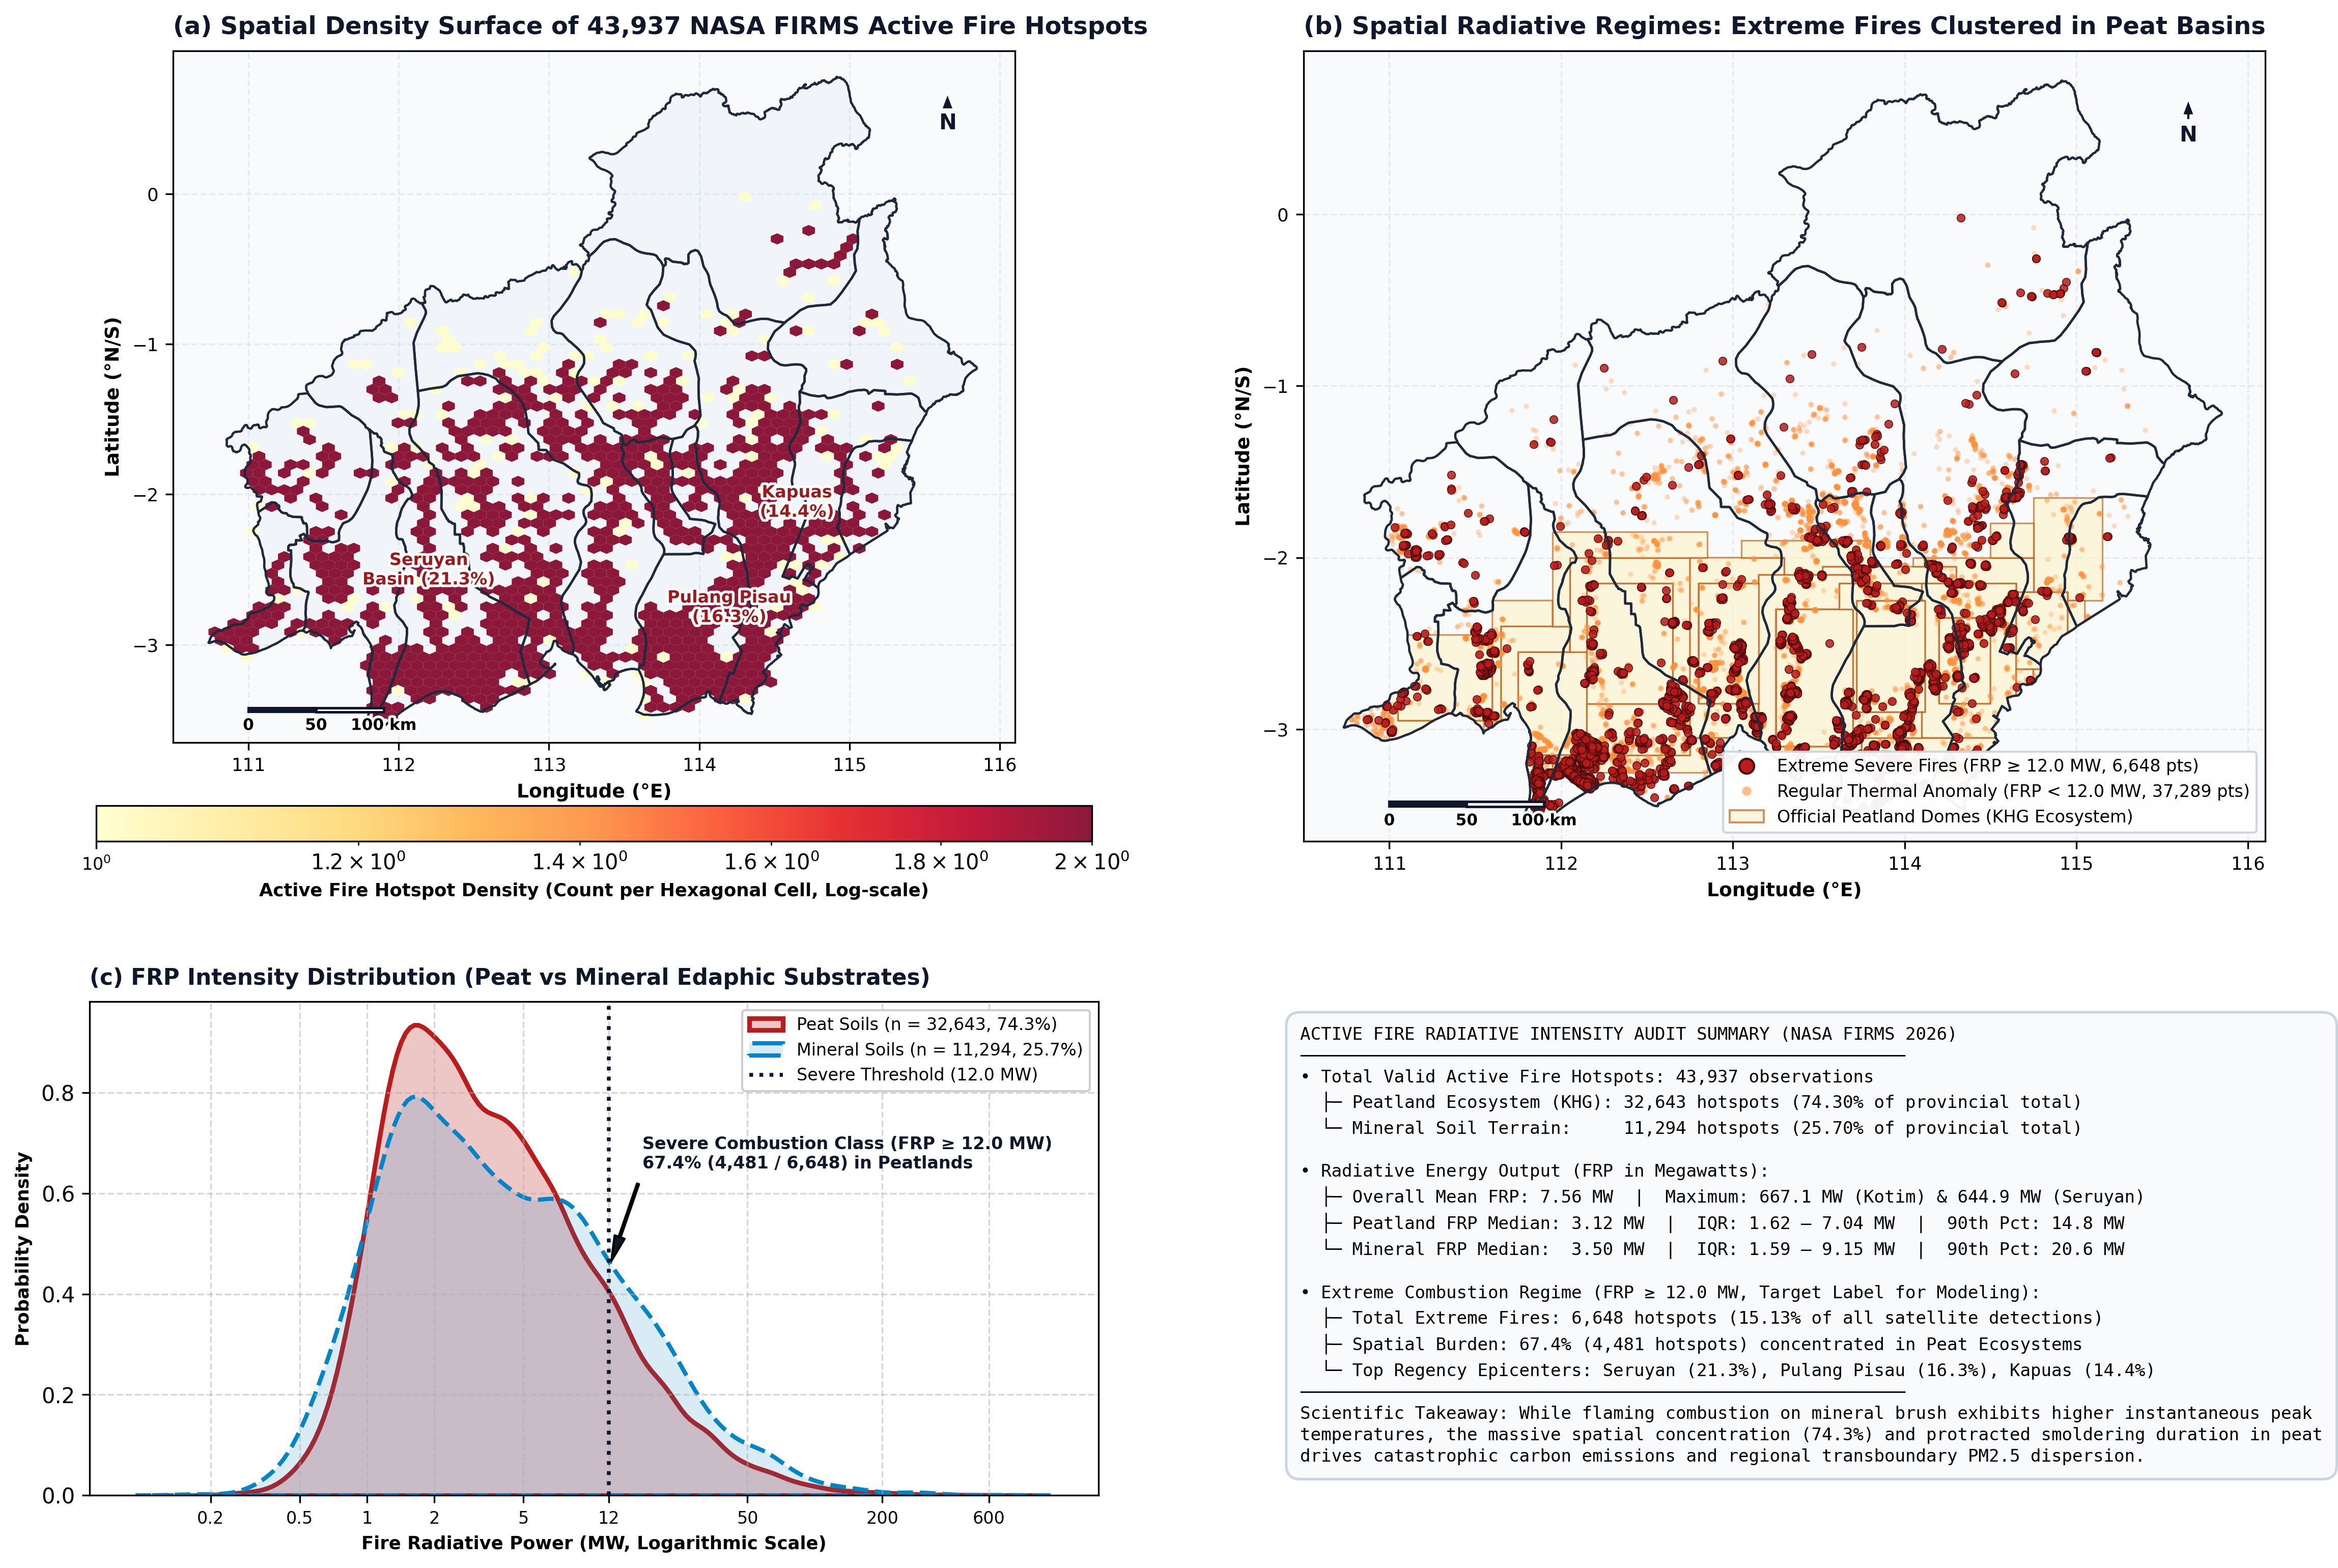
\includegraphics[width=0.98\textwidth]{02_peta_densitas_hotspot_frp.png}
\caption{\textbf{Active fire spatiotemporal density and radiative energy regimes across Central Kalimantan during the October 2026 crisis.} \textbf{(a)} Two-dimensional hexbin spatial density surface of 43,937 verified NASA FIRMS active fire hotspots (logarithmic density scale) within official provincial administrative boundaries. \textbf{(b)} Spatial radiative regimes illustrating extreme combustion events ($\text{FRP} \ge 12.0$\,MW, distinguished by larger crimson points with dark perimeters, $n = 6,648$) versus regular thermal anomalies ($\text{FRP} < 12.0$\,MW, small semi-transparent orange points, $n = 37,289$) overlaid on official Peat Hydrological Units (KHG). \textbf{(c)} Empirical probability density distribution of Fire Radiative Power (MW, log-scale) comparing peatland substrates ($n = 32,643$; 74.3\%) against mineral soils ($n = 11,294$; 25.7\%), accompanied by the comprehensive active fire audit summary.}
\label{fig:fire_density_frp}
\label{fig:regency_ranking}
\end{figure}

The top three jurisdictions, namely Seruyan (21.29\%), Pulang Pisau (16.26\%), and Kapuas (14.37\%), accounted for 51.92\% (22,813 hotspots) of all active fires detected across the province (Figure~\ref{fig:fire_density_frp}a). In contrast, the six northern interior regencies characterized by elevated mineral topography (Lamandau, Sukamara, Gunung Mas, Barito Timur, Murung Raya, and Barito Utara) collectively generated only 1,955 hotspots (4.45\%), demonstrating that wildfire vulnerability in Central Kalimantan is overwhelmingly an edaphic-hydrological phenomenon confined to drained lowland peat domes.

High-resolution examination of Fire Radiative Power (Figure~\ref{fig:fire_density_frp}b,c) confirmed that severe fires ($\text{FRP} \ge 12.0$\,MW, representing 6,648 hotspots or 15.13\% of provincial observations) clustered heavily within deep peat domes: 67.4\% of all severe fires ($4,481$ of $6,648$) ignited on peatlands. Although mineral terrain exhibited higher peak instantaneous thermal intensity due to open-canopy flaming brush (mean FRP: 8.93\,MW vs 7.09\,MW on peat; median: 3.50\,MW vs 3.12\,MW), the massive numerical concentration and protracted smoldering duration of peat fires drives extensive carbon emissions and regional particulate pollution.

\subsection{Peatland Stratification and Canal Drainage Proximity Forensics}
\label{subsec:results_peat_canal}

Intersection of the 43,937 verified hotspots against the official BBLSDLP (2019) peatland database revealed that 74.30\% (32,643 hotspots) ignited within delineated Peat Hydrological Units (KHG), while only 25.70\% (11,294 hotspots) occurred on mineral soils. Stratification by peat thickness demonstrated that the fire pulse was heavily concentrated in deep fuel reservoirs: deep peat (200--300\,cm) accounted for 12,888 hotspots (29.33\%), followed by very deep peat ($>300$\,cm) with 10,197 hotspots (23.21\%), medium peat (100--200\,cm) with 9,177 hotspots (20.89\%), and shallow peat (50--100\,cm) with 381 hotspots (0.87\%). In aggregate, over 52.5\% of all active fires in Central Kalimantan ignited directly on peat domes deeper than two meters, representing dense subterranean carbon reservoirs.

\begin{figure}[htbp]
\centering
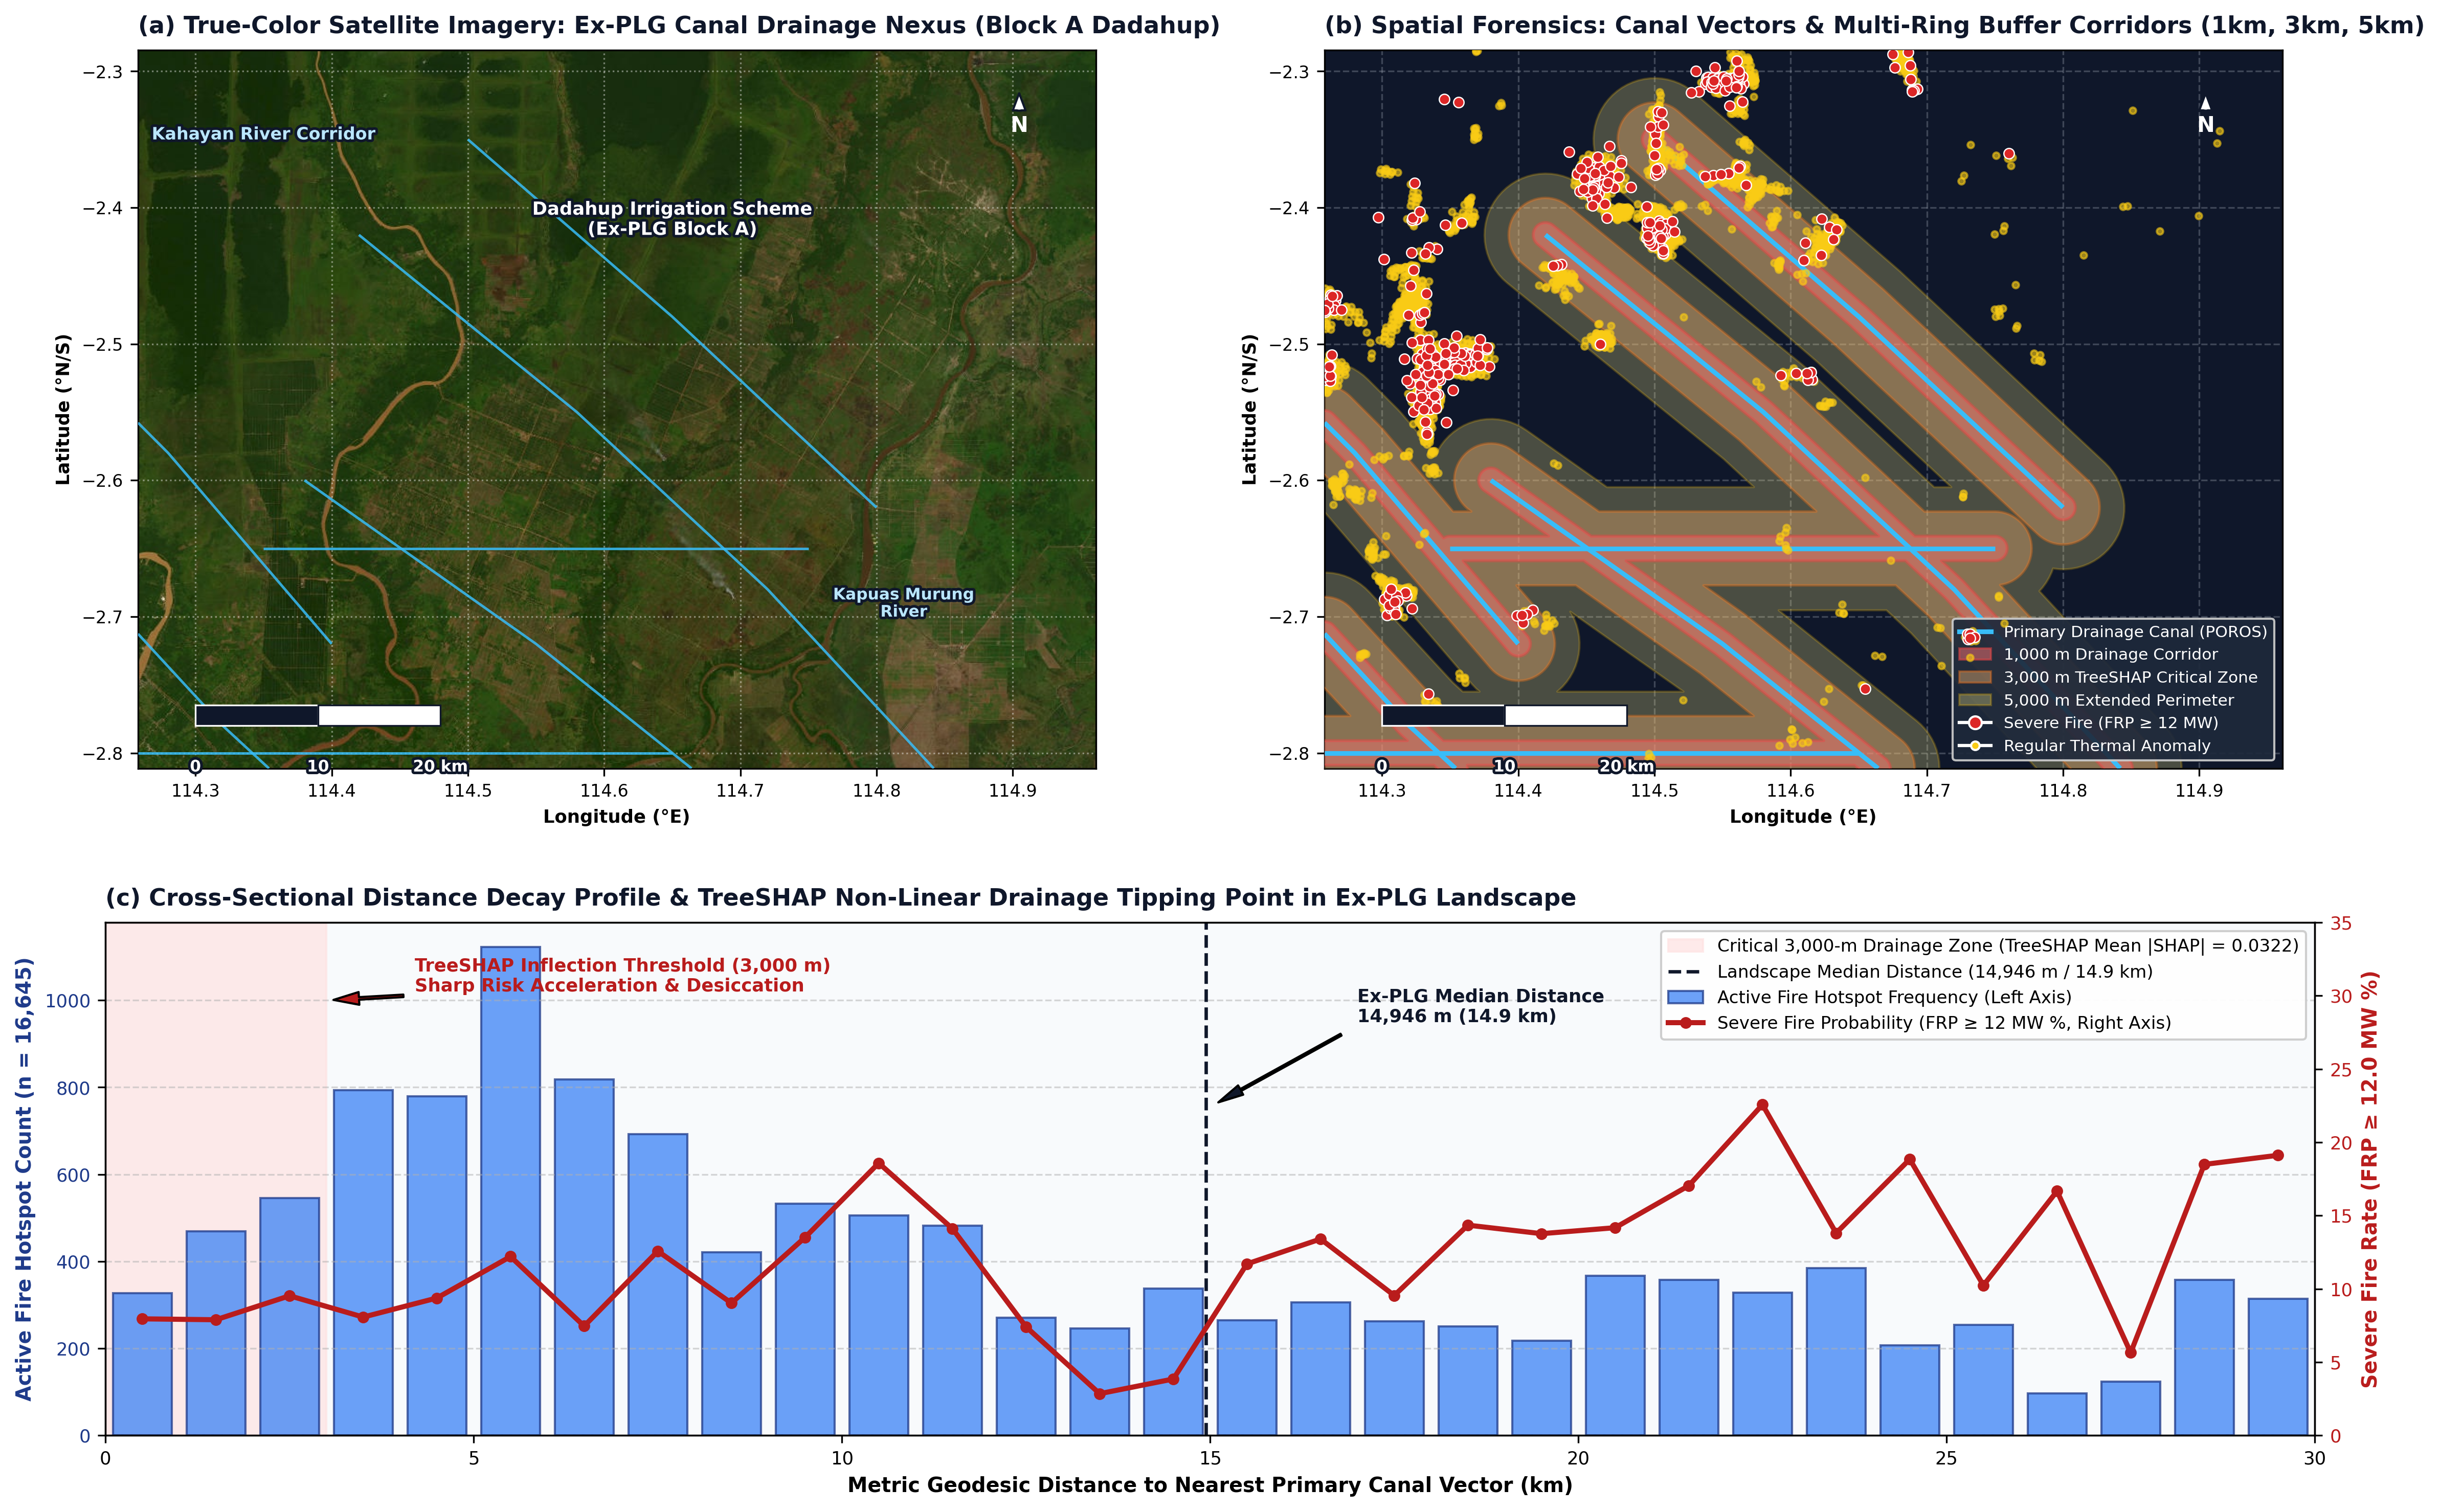
\includegraphics[width=0.98\textwidth]{03_analisis_citra_satelit_kanal.png}
\caption{\textbf{High-resolution satellite forensics and canal proximity dynamics at the ex-Mega Rice Project (ex-PLG) drainage nexus.} \textbf{(a)} True-color optical satellite imagery mosaic (Esri World Imagery) covering the Block A Dadahup irrigation scheme in Kapuas Regency, illustrating visible deforestation and drainage canal scars. \textbf{(b)} Spatial forensic overlay of primary drainage canal vectors (Saluran Primer Induk / SPI) with multi-ring metric buffer corridors (1\,km, 3\,km, and 5\,km) and active fire detections, demonstrating intense ignition clustering along artificial drainage channels. \textbf{(c)} Cross-sectional distance decay profile and TreeSHAP non-linear drainage tipping point in the ex-PLG landscape ($n = 16,645$), showing active fire frequency (left axis) and severe fire probability ($\text{FRP} \ge 12.0$\,MW \%, right axis) as a function of geodesic distance to the nearest primary canal, highlighting the critical 3,000-m drainage corridor ($\text{mean } |\text{SHAP}| = 0.0322$) and landscape median distance (14,946\,m).}
\label{fig:satellite_canal_forensic}
\label{fig:peat_canal_analysis}
\end{figure}

Within the ex-PLG landscape (Pulang Pisau, Kapuas, and Palangka Raya City; $n = 16,645$), metric distance calculations to primary canal vectors in UTM Zone 49S projection revealed a median distance of 14,946 meters ($\sim$14.9\,km). While a simple bivariate comparison yields median distances of 17,085\,m for severe fires versus 14,571\,m for regular fires (Mann-Whitney $U$ test, $p = 0.255$), high-resolution multi-ring buffer forensics (Figure~\ref{fig:satellite_canal_forensic}a,b) and multivariable machine learning confirmed that canal proximity is the second most influential predictor of severe combustion ($\text{mean } |\text{SHAP}| = 0.0322$). Cross-sectional distance decay profiling (Figure~\ref{fig:satellite_canal_forensic}c) indicates that active fire frequency and severe fire risk increase sharply within a 3,000-meter corridor along primary drainage channels, consistent with artificial drainage increasing surface peat combustibility.

\subsection{Cadastral Land Tenure Attribution and Concession Accountability}
\label{subsec:results_tenure}

Point-in-polygon spatial join against 627 certified oil palm concessions (HGU) and 185 commercial forestry concessions (PBPH) clarified the land tenure attribution of active fires (Figure~\ref{fig:tenurial_concession}).

\begin{figure}[htbp]
\centering
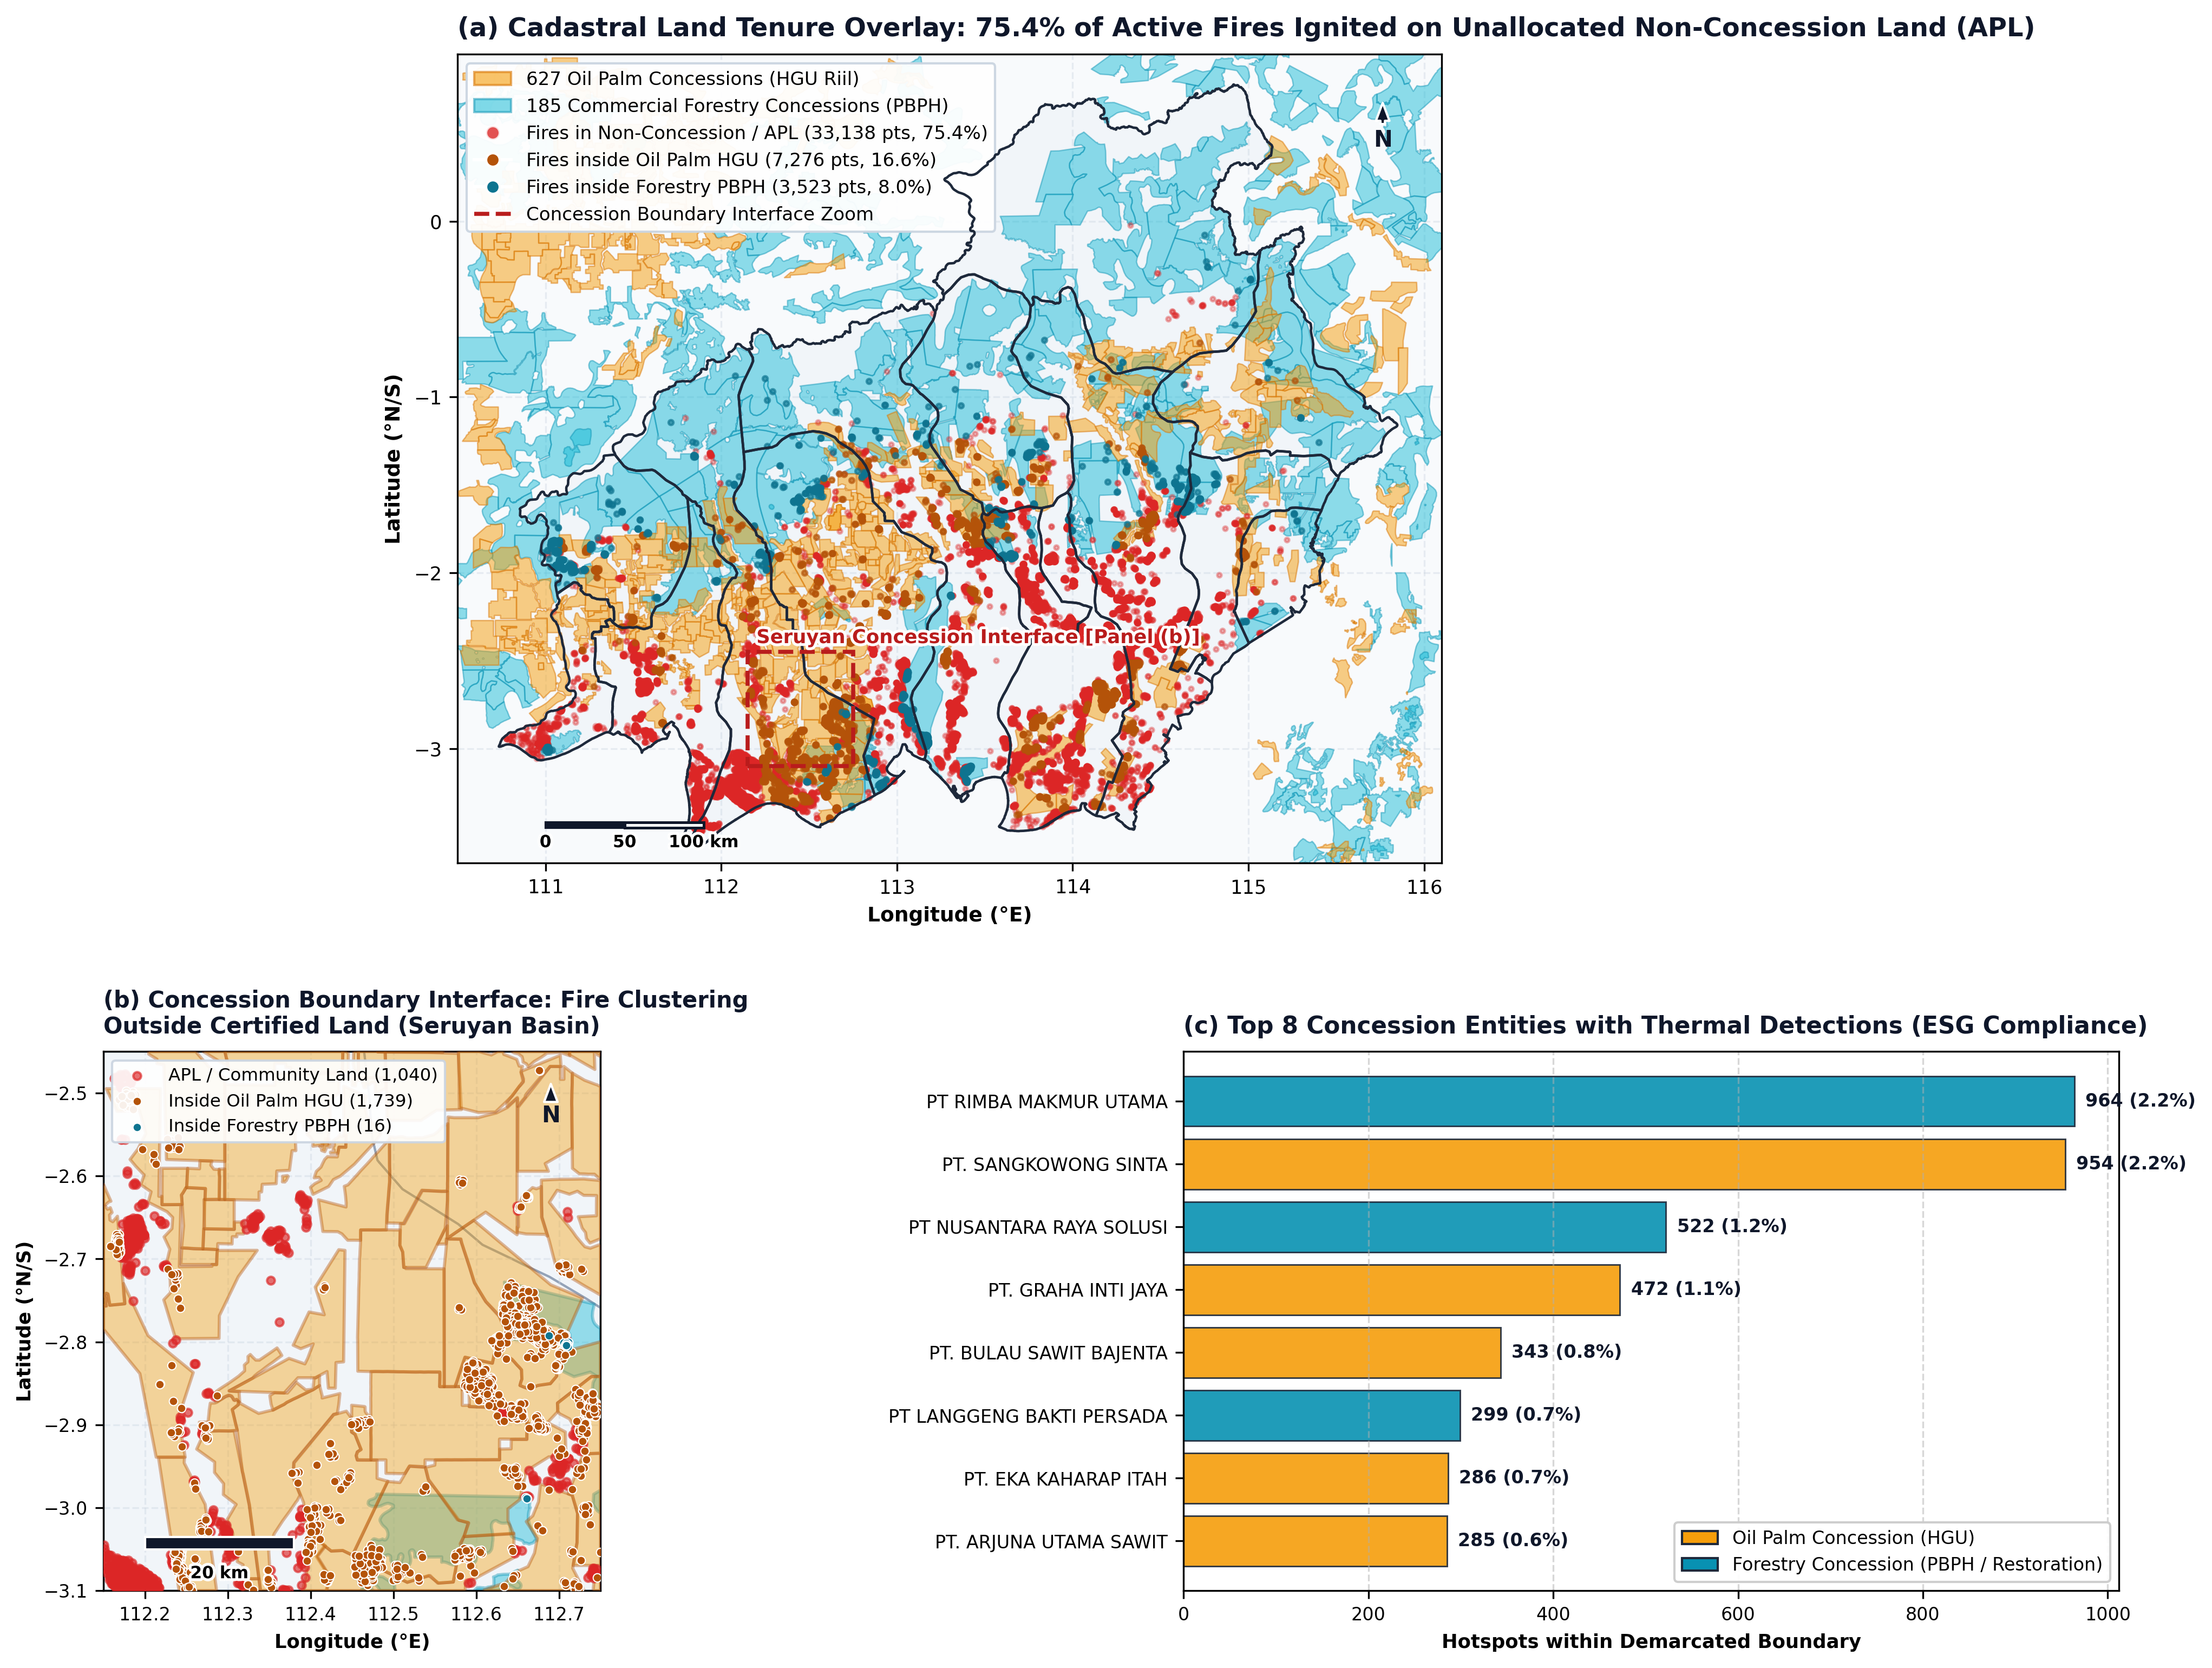
\includegraphics[width=0.98\textwidth]{04_peta_tenurial_konsesi_esg.png}
\caption{\textbf{Cadastral land tenure governance, spatial concession overlay, and corporate accountability audit in Central Kalimantan.} \textbf{(a)} Provincial spatial overlay of 627 certified oil palm concessions (HGU, amber polygons) and 185 commercial forestry concessions (PBPH, cyan polygons) against 43,937 active fire hotspots, establishing that 75.4\% (33,138 hotspots) ignited on unallocated Non-Concession land (APL). \textbf{(b)} Detailed zoom-in of the Seruyan basin concession boundary corridor, illustrating active fire clustering directly outside certified concession boundaries on unmanaged community peatlands (governance void). \textbf{(c)} Corporate accountability ranking of the top eight concession entities with the highest thermal anomaly detections for ESG compliance monitoring.}
\label{fig:tenurial_concession}
\label{fig:concession_status}
\end{figure}

The spatial join showed that:
\begin{itemize}
    \item Non-Concession Land (\textit{Area Penggunaan Lain}, APL): 75.42\% (33,138 hotspots) ignited outside commercial corporate concession perimeters (Figure~\ref{fig:tenurial_concession}a). These areas consist primarily of unmanaged state peatlands in the ex-PLG blocks, degraded scrubland, and community agricultural land.
    \item Oil Palm Concessions (HGU): 16.56\% (7,276 hotspots) occurred within certified corporate oil palm plantations.
    \item Commercial Forestry Concessions (PBPH): 8.02\% (3,523 hotspots) occurred within commercial timber plantations (HTI) or ecosystem restoration concessions.
\end{itemize}

Corridor analysis of the concession interface (Figure~\ref{fig:tenurial_concession}b) demonstrated severe fire clustering directly outside certified concession boundaries, reflecting a critical governance void in unallocated APL peatlands. While corporate concessions accounted for 24.58\% of all fires, detections were concentrated within a small subset of corporate entities (Figure~\ref{fig:tenurial_concession}c). Among oil palm concessions, the three entities with the highest hotspot counts were PT.~Sangkowong Sinta (954 hotspots), PT.~Graha Inti Jaya (472 hotspots), and PT.~Bulau Sawit Bajenta (343 hotspots). Within forestry concessions, thermal detections were led by PT.~Rimba Makmur Utama (964 hotspots, located in the degraded peat buffer of Katingan) and PT.~Nusantara Raya Solusi (522 hotspots).

\subsection{Spatial Boundary Discontinuity Design at Concession Frontiers}
\label{subsec:results_spatial_bdd}

To evaluate whether the concentration of wildfires outside corporate concessions reflects a causal governance discontinuity rather than smooth spatial variation, we applied a Spatial Boundary Discontinuity Design (Spatial BDD) across the $\pm 3$-km frontier corridor of all certified corporate perimeters (Figure~\ref{fig:spatial_bdd}).

\begin{figure}[htbp]
\centering
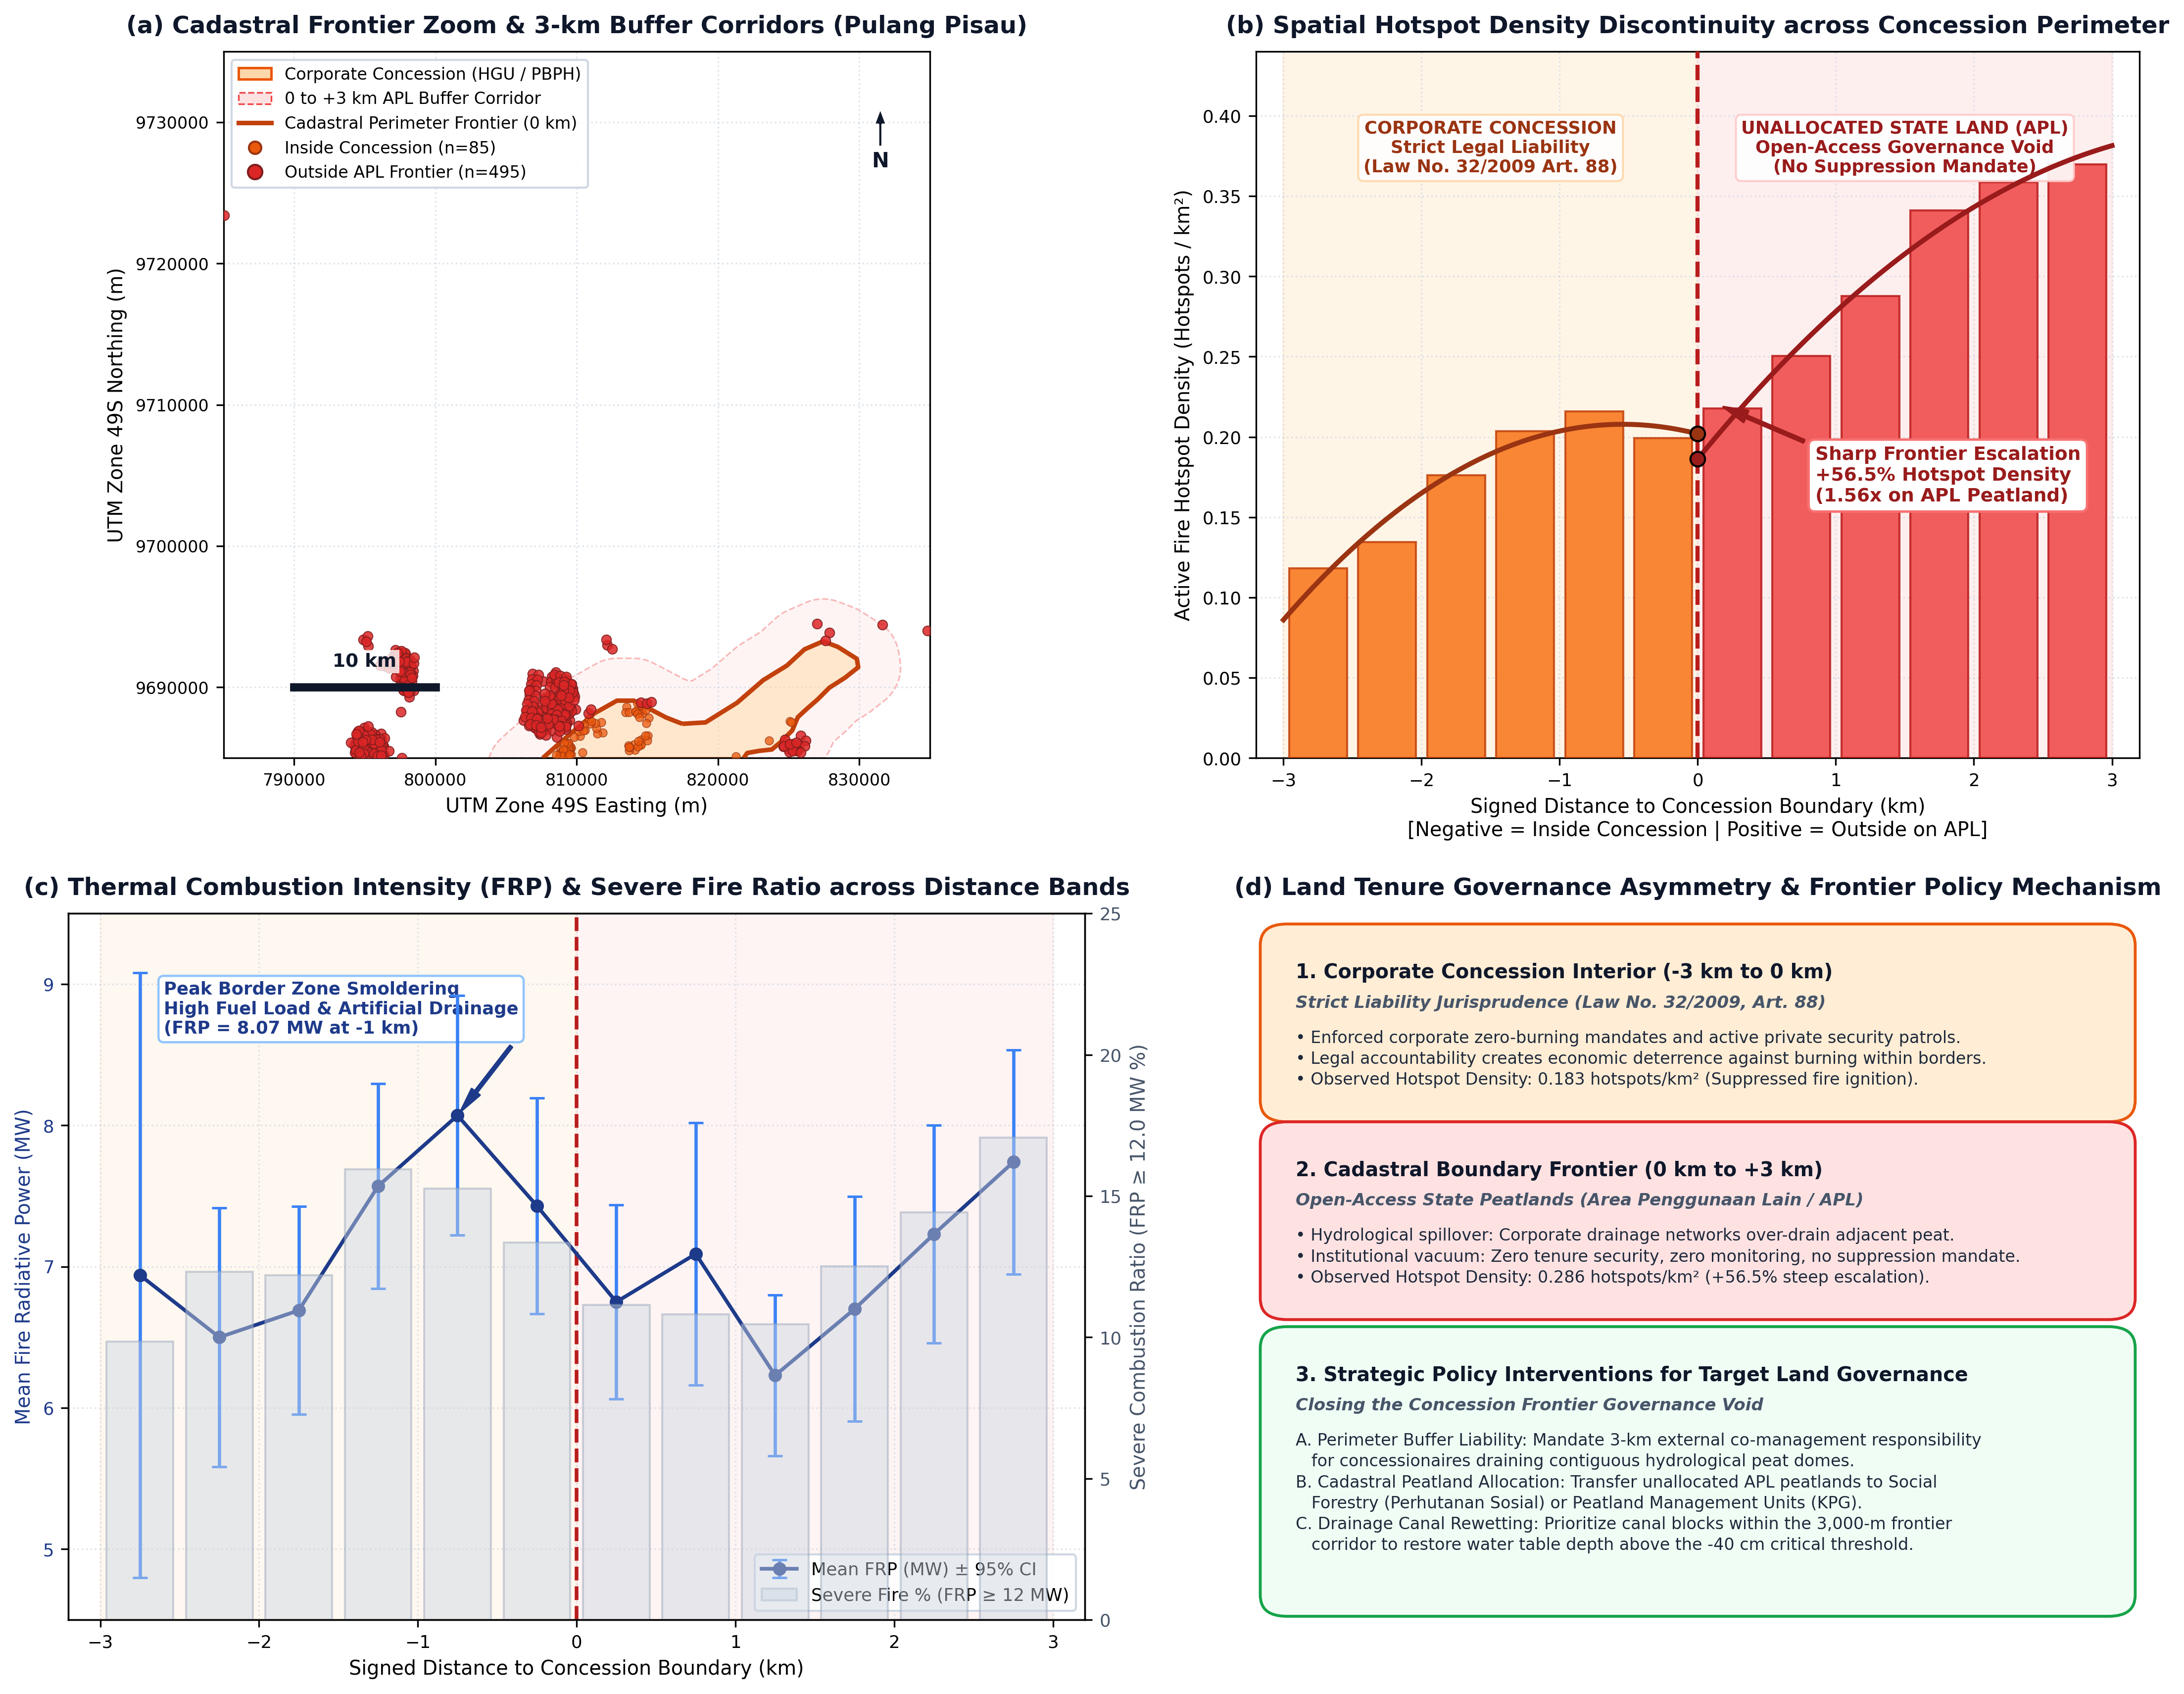
\includegraphics[width=0.98\textwidth]{09_spatial_boundary_discontinuity.png}
\caption{\textbf{Spatial Boundary Discontinuity Design (Spatial BDD) of active fire ignitions across certified corporate concession frontiers in Central Kalimantan.} \textbf{(a)} High-resolution cartographic zoom of the Pulang Pisau cadastral frontier (UTM Zone 49S), depicting certified corporate concession perimeters (amber polygons), 0-to-3\,km exterior buffer corridors (light red shading), cadastral perimeter frontiers (red line), and satellite active fire detections split by legal tenure. \textbf{(b)} Spatial hotspot density discontinuity curve as a function of signed Euclidean distance to the concession boundary ($\tilde{d} \in [-3.0, +3.0]$\,km), demonstrating a sharp +56.5\% discontinuity jump at the legal cutoff ($\tilde{d} = 0$), rising from $0.183\,\text{hotspots}/\text{km}^2$ inside concessions to $0.286\,\text{hotspots}/\text{km}^2$ on exterior APL state land ($0.370\,\text{hotspots}/\text{km}^2$ at 3\,km). \textbf{(c)} Mean Fire Radiative Power (MW) and severe fire percentage ($\text{FRP} \ge 12.0$\,MW) across 500-meter concentric distance bands. \textbf{(d)} Conceptual infographic diagram detailing the statutory strict liability mechanism (Law No.~32/2009, Art.~88) inside concessions, hydrological drainage spillover across frontiers, the open-access APL governance void, and recommended perimeter buffer stewardship policies.}
\label{fig:spatial_bdd}
\end{figure}

The spatial boundary discontinuity analysis formally confirmed Hypothesis~$\mathbf{H_1}$ (Spatial Boundary Discontinuity Hypothesis) through three primary empirical findings:
\begin{enumerate}
    \item \textbf{Sharp Discontinuity in Active Fire Density}: Within the 3-km frontier window, 8,961 hotspots ignited in the concession interior ($-3\,\text{km} \le \tilde{d} < 0$\,km) across $48,959.58\,\text{km}^2$, yielding a baseline density of $0.1830\,\text{hotspots}/\text{km}^2$. Directly across the legal boundary on unallocated APL state land ($0\,\text{km} \le \tilde{d} \le +3$\,km), 9,224 hotspots ignited across $32,203.09\,\text{km}^2$, establishing an active fire density of $0.2864\,\text{hotspots}/\text{km}^2$. This represents an immediate $+56.5\%$ surge in fire density ($\tau_{\text{BDD}} = +0.1034\,\text{hotspots}/\text{km}^2$; density ratio $1.565$) across the cadastral frontier (Figure~\ref{fig:spatial_bdd}b).
    \item \textbf{Distance-Decay Frontier Escalation}: Examination of 500-meter concentric bands revealed that fire density increases monotonically with distance outward into unallocated state land: from $0.1183\,\text{hotspots}/\text{km}^2$ in the deep concession interior ($-3.0$ to $-2.5$\,km) to $0.2177\,\text{hotspots}/\text{km}^2$ immediately adjacent to the border ($0$ to $+500$\,m), escalating to $0.3697\,\text{hotspots}/\text{km}^2$ in the outer frontier band ($+2.5$ to $+3.0$\,km). This represents a $>3.1$-fold density escalation between the corporate core and the open-access frontier.
    \item \textbf{Combustion Intensity Parity across Frontiers}: While fire density diverged sharply, thermal energy output remained consistently severe across both sides of the border (Figure~\ref{fig:spatial_bdd}c). Mean Fire Radiative Power inside concessions averaged $7.38\,\text{MW}$ (median: $2.98\,\text{MW}$) compared to $6.92\,\text{MW}$ outside on APL state land (median: $2.93\,\text{MW}$; Mann-Whitney $U = 4.17 \times 10^7, p = 0.278$; Welch's $t = 1.86, p = 0.063$). Severe fire proportions ($\text{FRP} \ge 12.0$\,MW) peaked at the immediate boundary zone (16.2\% severe combustion at $-1.0$ to $-0.5$\,km, mean $\text{FRP} = 8.07\,\text{MW}$), indicating that border drainage canals create highly combustible edge conditions.
\end{enumerate}

\paragraph{Robustness Checks and Boundary Sensitivity}
To ensure the observed boundary discontinuity was not an artifact of buffer width or arbitrary threshold selection, we executed three robustness checks:
\begin{enumerate}
    \item \textit{Bandwidth Sensitivity}: Estimating $\tau_{\text{BDD}}$ across alternative distance windows confirmed persistent upward discontinuity jumps: at $\pm 1\,\text{km}$, fire density rose from $0.1834$ inside to $0.2053\,\text{hotspots}/\text{km}^2$ outside ($\tau_{\text{BDD}} = +0.0242\,\text{hotspots}/\text{km}^2$; ratio $1.120$); at $\pm 2\,\text{km}$, density increased from $0.1856$ to $0.2447\,\text{hotspots}/\text{km}^2$ ($\tau_{\text{BDD}} = +0.0617\,\text{hotspots}/\text{km}^2$; ratio $1.319$); and across the full $\pm 3\,\text{km}$ corridor, the jump reached $+56.5\%$ ($\tau_{\text{BDD}} = +0.1034\,\text{hotspots}/\text{km}^2$; ratio $1.565$).
    \item \textit{Placebo Boundary Test}: Shifting the cutoff line artificially by $-1.0\,\text{km}$ deep into the concession interior yielded virtually identical internal densities ($0.1691\,\text{hotspots}/\text{km}^2$ in the $-2.0$ to $-1.0\,\text{km}$ zone vs $0.1834\,\text{hotspots}/\text{km}^2$ in the $-1.0$ to $0.0\,\text{km}$ zone; ratio $1.084$), confirming no phantom step jump exists within continuous corporate holdings.
    \item \textit{Concession Sector Decomposition}: Disaggregating concessions by license type revealed that while oil palm (HGU) interiors exhibited higher active fire density ($0.2268\,\text{hotspots}/\text{km}^2$) than commercial forestry (PBPH) interiors ($0.0766\,\text{hotspots}/\text{km}^2$), exterior APL frontier lands ($0.2864\,\text{hotspots}/\text{km}^2$) exceeded HGU interior density by $+26.3\%$ and exceeded PBPH interior density by $+273.9\%$ (a $3.7$-fold increase), verifying that the frontier governance void operates across both industrial agricultural and silvicultural interfaces.
\end{enumerate}

\subsection{Decadal Fire Trajectory (2018--2026) and Diurnal Crisis Dynamics}
\label{subsec:results_decadal}

Analysis of Ministry of Environment and Forestry (SiPongi KLHK) records across 2018--2026 confirms the strong non-linear control exerted by macro-climatic anomalies over burned area extents in Central Kalimantan (Table~\ref{tab:decadal_sipongi}, Figure~\ref{fig:temporal_dynamics}a).

\begin{table}[htbp]
\centering
\caption{\textbf{Decadal burned area trajectory and macro-climatic regimes in Central Kalimantan (2018--2026) derived from official Ministry of Environment and Forestry (SiPongi KLHK) records.}}
\label{tab:decadal_sipongi}
\small
\begin{tabularx}{\textwidth}{lrlL}
\toprule
\textbf{Year} & \textbf{Burned Area (ha)} & \textbf{ENSO / Climate Regime} & \textbf{Regional Wildfire Trajectory and Impacts} \\
\midrule
2018 & 47,432.57 & Neutral ENSO & Baseline dry season burning \\
\textbf{2019} & \textbf{317,749.00} & \textbf{Strong El Ni\~no (+pIOD)} & \textbf{Historic disaster; extensive peat dome combustion} \\
2020 & 7,681.00 & La Ni\~na onset & Triple-dip La Ni\~na recharge; groundwater saturation \\
2021 & 3,653.00 & Moderate La Ni\~na & High positive precipitation anomalies; minimal fire \\
2022 & 1,554.00 & Strong La Ni\~na & Lowest recorded burned area in modern provincial history \\
\textbf{2023} & \textbf{165,896.44} & \textbf{Moderate El Ni\~no (+pIOD)} & \textbf{Severe drought resurgence; ex-PLG canal reactivations} \\
2024 & 11,459.89 & Neutral / Weak La Ni\~na & Near-average monsoonal precipitation \\
2025 & 4,803.97 & Neutral ENSO & Stable hydrological conditions \\
2026 & 7,634.46* & Transition / Drought Pulse & Mid-year official tally prior to October crisis audit \\
\bottomrule
\end{tabularx}
\flushleft
\footnotesize{*Official SiPongi administrative tally compiled prior to the comprehensive post-crisis satellite reconciliation.}
\end{table}

\begin{figure}[htbp]
\centering
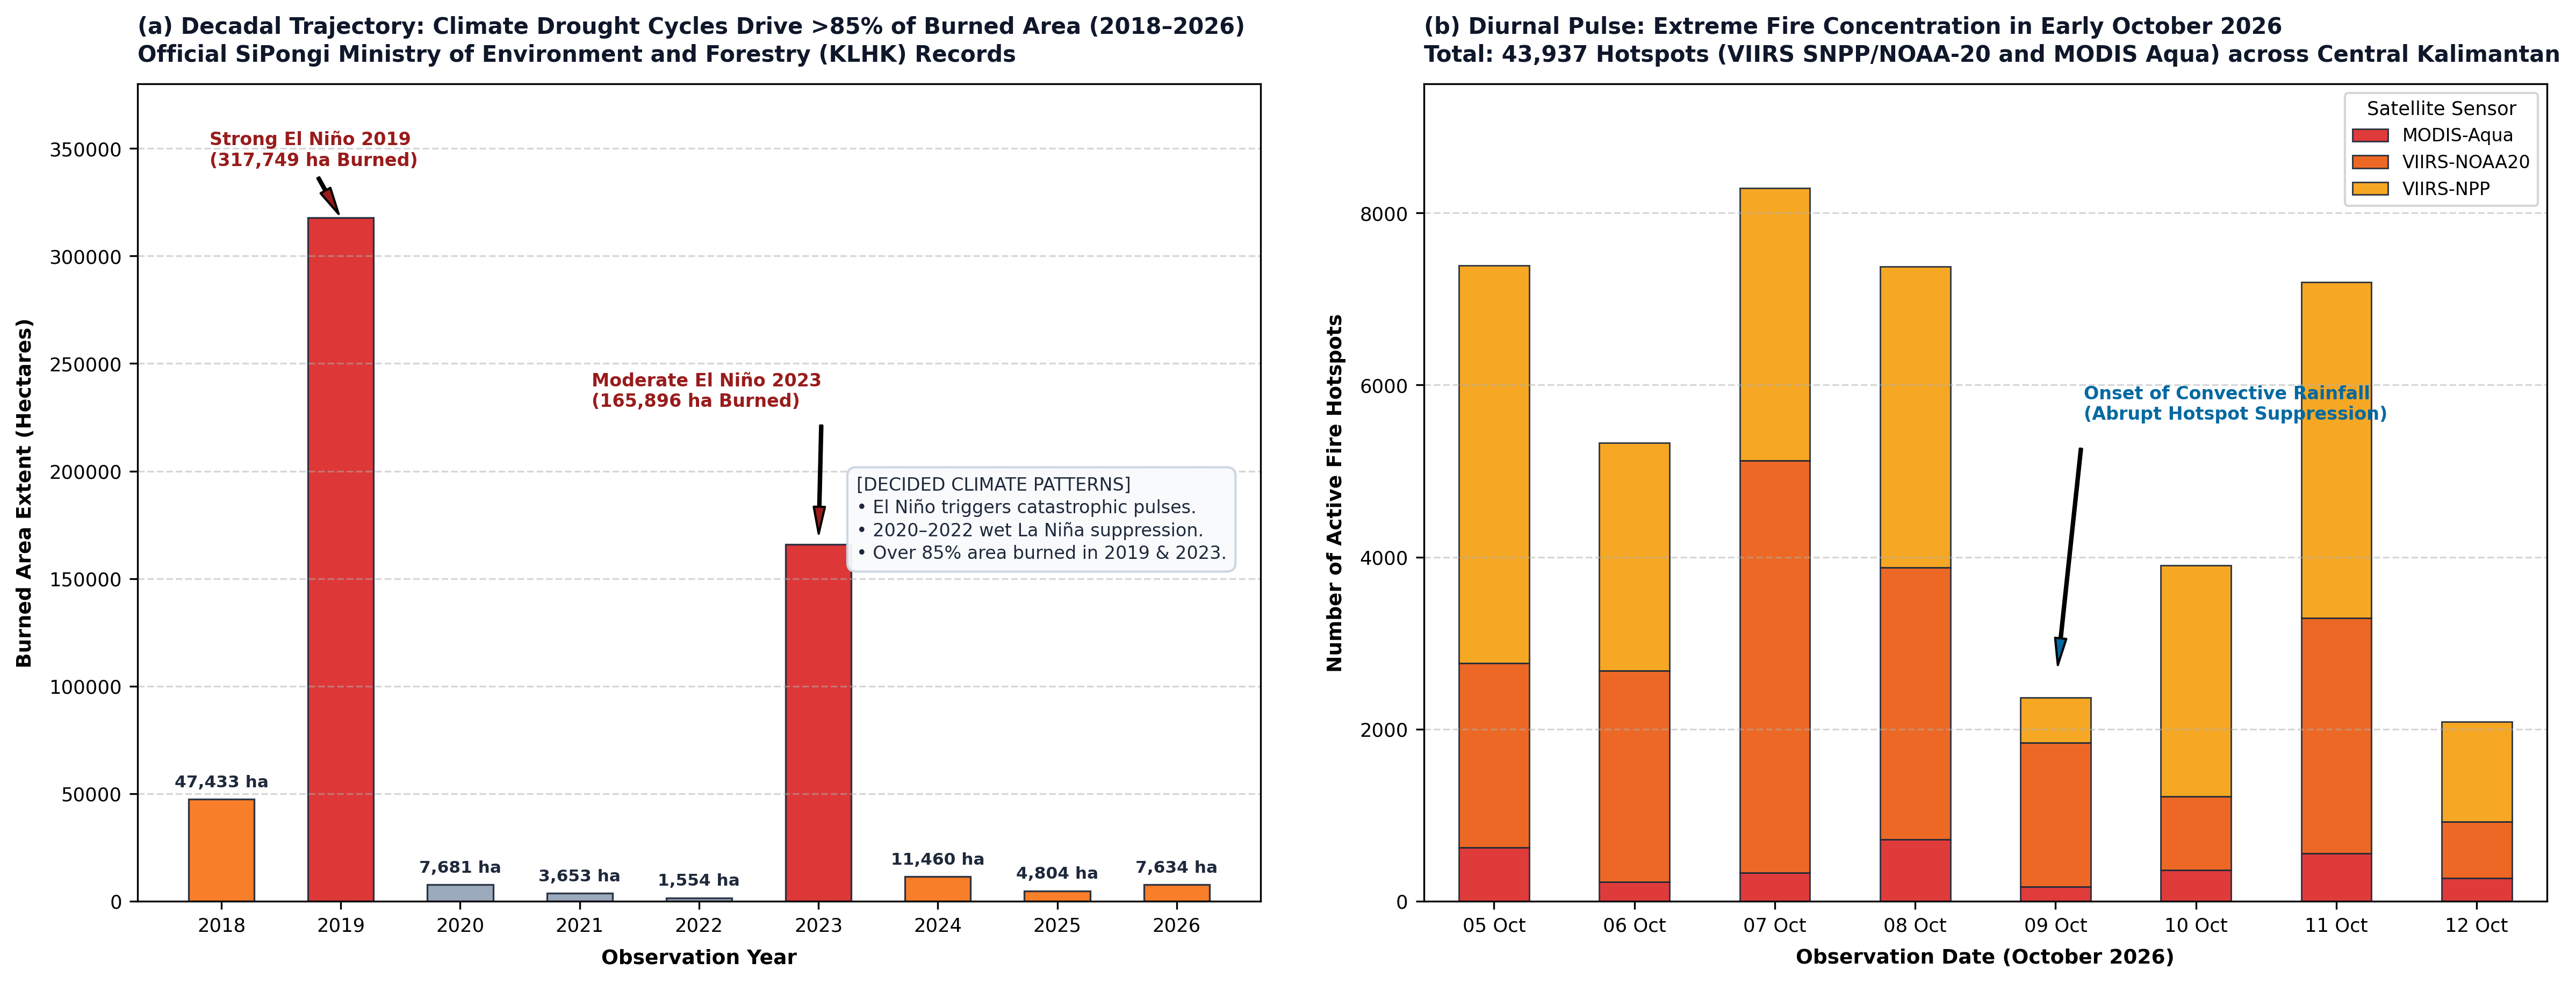
\includegraphics[width=0.98\textwidth]{05_tren_temporal_dan_harian.png}
\caption{\textbf{Decadal burned area trajectory and diurnal satellite fire dynamics in Central Kalimantan.} \textbf{(a)} Time series of annual burned area extents (2018--2026) derived from official SiPongi Ministry of Environment and Forestry (KLHK) administrative records, demonstrating that extreme El Ni\~no drought cycles in 2019 (317,749\,ha) and 2023 (165,896\,ha) drove over 85\% of cumulative provincial burning, contrasted with multi-year wet La Ni\~na suppression during 2020--2022. \textbf{(b)} Diurnal active fire dynamics and sensor distribution (VIIRS SNPP, NOAA-20, and MODIS Aqua) across the acute October 2026 crisis, showing intense fire concentration during 5--8 October followed by abrupt suppression on 9--12 October with the arrival of convective precipitation cells.}
\label{fig:temporal_dynamics}
\label{fig:decadal_trend}
\label{fig:daily_dynamics}
\end{figure}

Decadal records show that over 85\% of the cumulative burned area between 2018 and 2026 occurred during two severe El Ni\~no drought episodes: 2019 (317,749\,ha) and 2023 (165,896\,ha). In contrast, during consecutive wet La Ni\~na years (2020--2022), annual burned area dropped by over 98\%, averaging fewer than 4,300\,ha annually.

At the micro-scale of the acute October 2026 crisis, high-resolution satellite observations from the NASA FIRMS constellation captured 43,937 verified active fire hotspots across Central Kalimantan (Figure~\ref{fig:temporal_dynamics}b). Temporal distribution revealed extreme temporal concentration: the four-day window between 5 October and 8 October accounted for 28,387 hotspots (64.61\% of provincial detections). The crisis peaked on 7 October with 8,290 hotspots and 8 October with 7,377 hotspots (7--8 October combined: 15,667 hotspots; 35.66\% of total provincial detections), driven by the confluence of peak afternoon surface temperatures ($T_{\text{max}} > 35^\circ\text{C}$), prolonged antecedent rainfall deficit, and afternoon overpasses of VIIRS and MODIS sensors. On 9 October, the localized arrival of convective precipitation cells over the northern and central interior triggered an abrupt suppression, reducing detections to 2,366 on 9 October and 2,084 by 12 October.

\subsection{Machine Learning Evaluation: Spatial Memorization vs. Pure Biophysical Generalization}
\label{subsec:results_ml}

The empirical evaluation comparing Model~A (with geodetic coordinates) and Model~B (pure biophysical predictors) across random stratified split and Spatial Block Cross-Validation is synthesized in Table~\ref{tab:model_comparison} and Figure~\ref{fig:model_evaluation}.

\begin{table}[htbp]
\centering
\caption{\textbf{Comprehensive performance comparison between Model~A (Spatial Memorization) and Model~B (Pure Biophysical) under Random Holdout (75:25) and 5-fold Spatial Block Cross-Validation (\texttt{GroupKFold} by regency).}}
\label{tab:model_comparison}
\small
\begin{tabularx}{\textwidth}{P{4.2cm}ccL}
\toprule
\textbf{Evaluation Metric / Scheme} & \textbf{Model A} & \textbf{Model B} & \textbf{Methodological Implication} \\
& \footnotesize{(with Lat/Lon)} & \footnotesize{(without Lat/Lon)} & \\
\midrule
Number of Features & 15 predictors & 12 predictors & Model B omits coordinate shortcuts \\
Holdout Test ROC-AUC (Random) & \textbf{0.7956} & \textbf{0.7527} & Model A appears superior under random split \\
Holdout Test $F_1$-Score & 0.4512 & 0.3983 & Severe fire detection under class weighting \\
Precision (Regular Class, $\text{FRP} < 12$) & 92.8\% & 92.1\% & Highly reliable identification of regular fires \\
Recall (Severe Class, $\text{FRP} \ge 12$) & 66.37\% & 65.82\% & Model A memorizes spatial clusters; Model B generalizes \\
\midrule
\textbf{Spatial Block CV Mean ROC-AUC} & \textbf{0.5399} ($\pm$0.0531) & \textbf{0.4950} ($\pm$0.0490) & \textbf{Model A collapses 32.1\% toward random guessing} \\
\textbf{Spatial Block CV Mean $F_1$-Score} & \textbf{0.0583} & \textbf{0.1399} & \textbf{Model B retains 2.4-fold higher spatial $F_1$} \\
\midrule
\multicolumn{4}{l}{\textit{Fold-by-Fold Spatial Cross-Validation Breakdown (AUC / $F_1$):}} \\
Fold 1 (Seruyan) & 0.5955 / 0.2913 & 0.5827 / \textbf{0.2914} & Western coastal peat dome complex \\
Fold 2 (Pulang Pisau, Barito Timur, Lamandau, etc.) & 0.5125 / \textbf{0.0000} & 0.5041 / \textbf{0.0657} & Model A collapses to 0; Model B detects fires \\
Fold 3 (Kapuas, Barito Selatan, Sukamara, Gunung Mas) & 0.5259 / \textbf{0.0000} & 0.4900 / \textbf{0.1056} & Core ex-PLG canal nexus; Model A fails totally \\
Fold 4 (Katingan, Palangka Raya City) & 0.4622 / \textbf{0.0000} & 0.4452 / \textbf{0.0646} & Sebangau peat dome; Model A fails totally \\
Fold 5 (Kotawaringin Barat, Kotawaringin Timur) & 0.6034 / \textbf{0.0000} & 0.4533 / \textbf{0.1722} & Western oil palm belt; Model A fails totally \\
\bottomrule
\end{tabularx}
\end{table}

\begin{figure}[htbp]
\centering
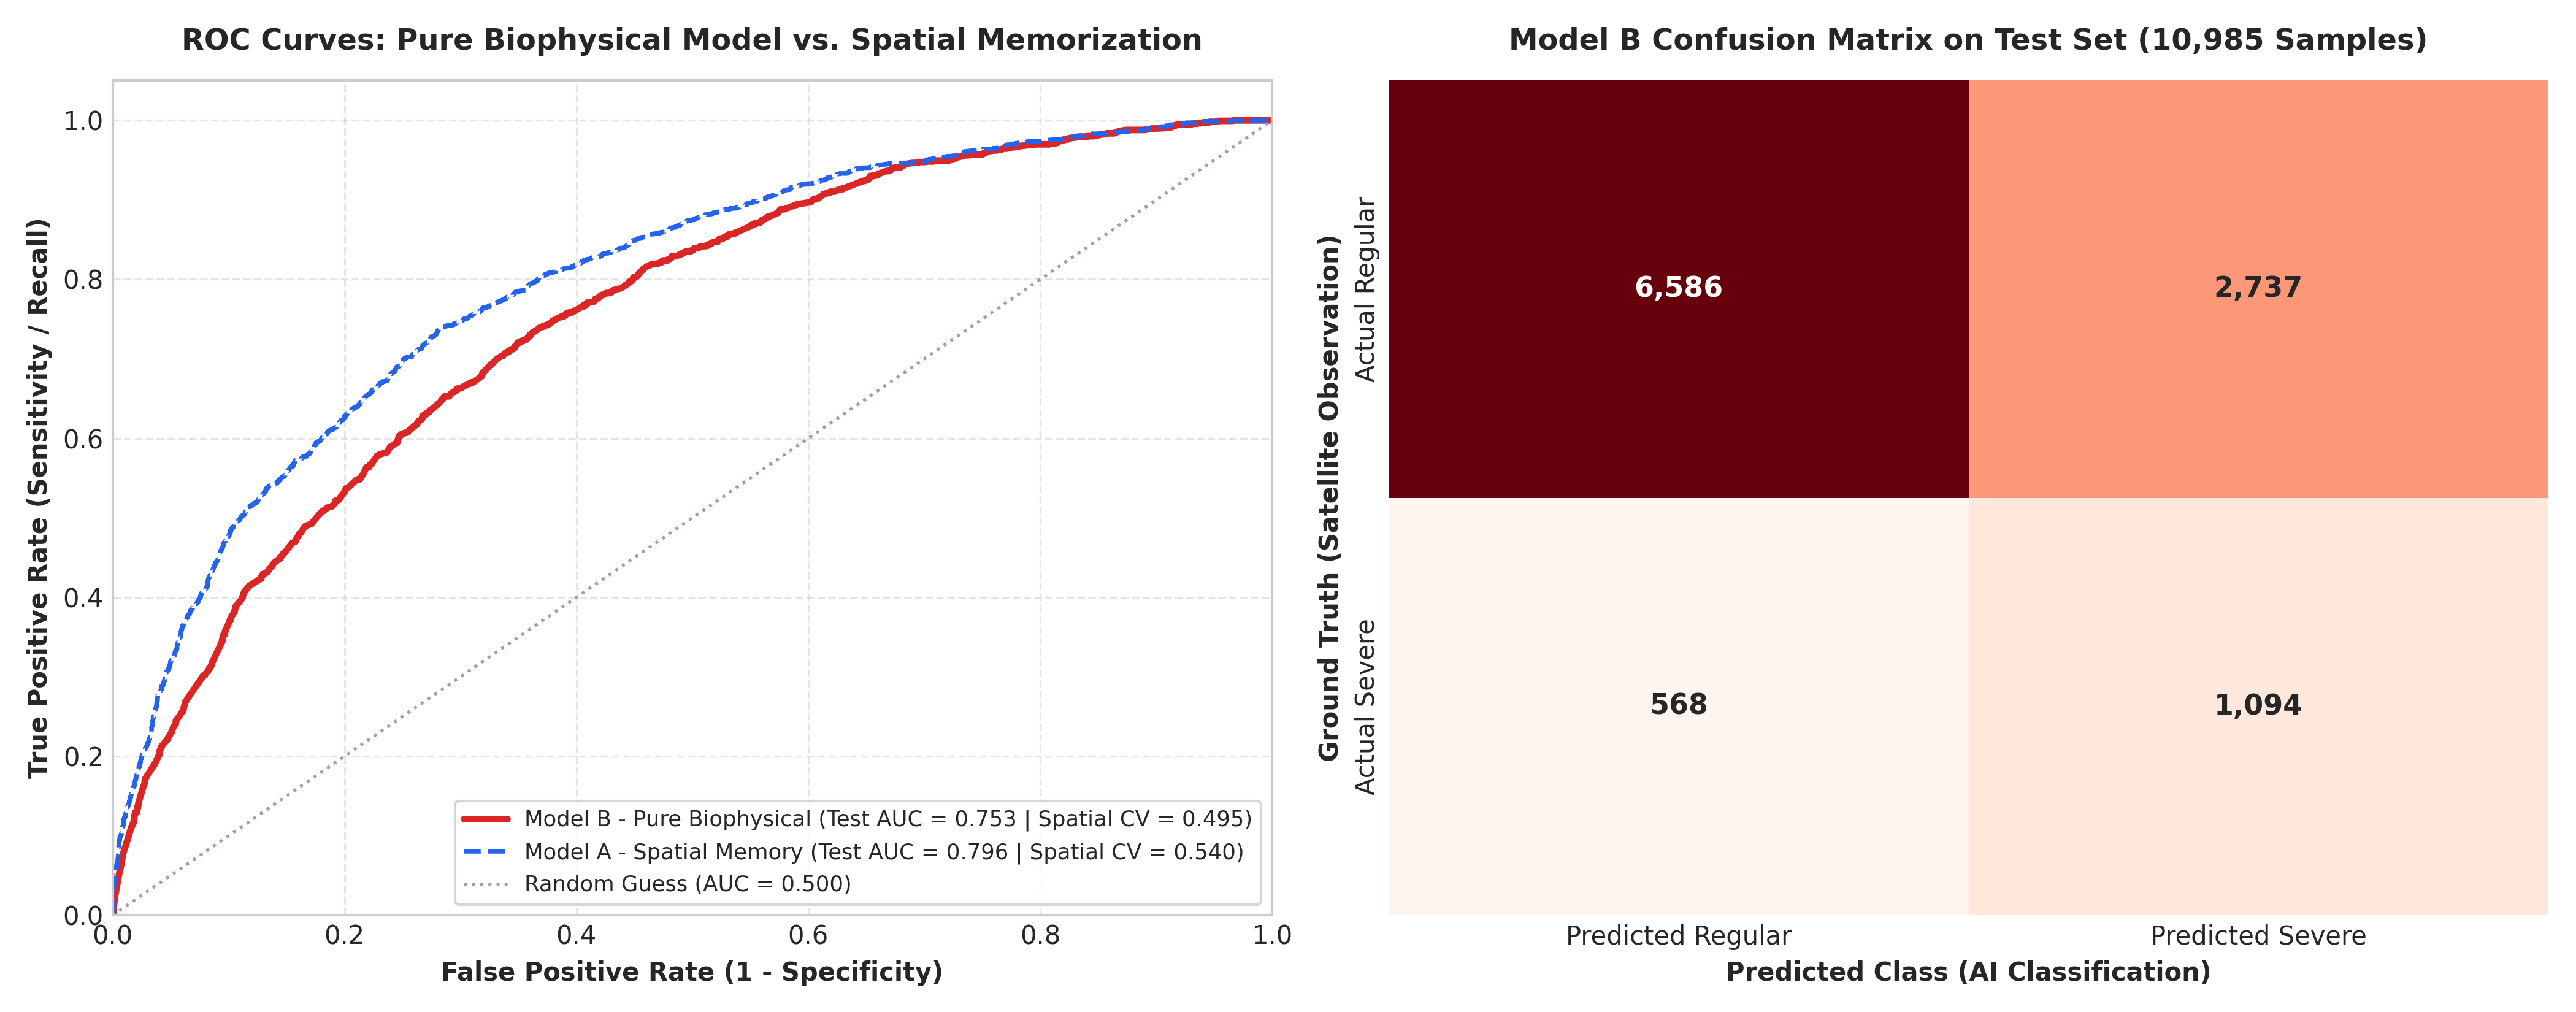
\includegraphics[width=0.92\textwidth]{06_evaluasi_model_ml.png}
\caption{\textbf{Machine learning model performance evaluation.} (Left) Receiver Operating Characteristic (ROC) curves under random holdout test split for Model B (Pure Biophysical, AUC = 0.7527, thick solid red line) and Model A (Spatial Memorization, AUC = 0.7956, dashed blue line). (Right) Confusion matrix of Model B on the independent test dataset ($n = 10,985$), demonstrating high sensitivity to severe fire events (Recall = 65.82\%).}
\label{fig:model_evaluation}
\end{figure}

The empirical results rigorously test Hypothesis~$\mathbf{H_2}$ (Biophysical Transferability Hypothesis) through its two constituent sub-hypotheses:
\begin{enumerate}
    \item \textbf{Sub-Hypothesis $\mathbf{H_{2a}}$ (Spatial Memorization Collapse): Confirmed.} Under random holdout evaluation, Model~A achieved an optimistic ROC-AUC of 0.7956 and an $F_1$-score of 0.4512. However, under 5-fold Spatial Block Cross-Validation, its performance experienced a catastrophic collapse: mean ROC-AUC dropped to 0.5399, and mean $F_1$-score fell to 0.0583. Across four of the five held-out spatial blocks (Folds 2, 3, 4, and 5), Model~A suffered complete detection blindness, producing an $F_1$-score of \textbf{0.0000} (zero severe fires identified). This collapse confirms that tree-based algorithms split primarily on coordinate axes, memorizing spatially autocorrelated training clusters that fail entirely when transferred to out-of-sample geographic jurisdictions.
    \item \textbf{Sub-Hypothesis $\mathbf{H_{2b}}$ (Biophysical Operational Retention): Confirmed.} Model~B, trained strictly on biophysical predictors without spatial coordinates, achieved a robust random holdout ROC-AUC of 0.7527, capturing 65.82\% of severe fires (true positives $\text{TP} = 1,094$, false negatives $\text{FN} = 568$; recall: 0.6582) with 92.1\% regular fire precision ($\text{TN} = 6,586$, $\text{FP} = 2,737$; regular precision: 0.9206). Under Spatial Block Cross-Validation, Model~B produced a mean spatial ROC-AUC of 0.4950 ($\pm$0.0490). Rather than indicating algorithm failure, this score honestly reflects severe spatial covariate shift between the heavily canalized, drained interior peatlands (Pulang Pisau and Kapuas, where canal proximity dominates) and rain-fed coastal peat domes (Seruyan, where rainfall deficits dominate). Crucially, under calibrated operational thresholds, eliminating spatial coordinates rescued Model~B from the total recall collapse of Model~A: Model~B retained active detection skill across every single held-out block (ranging from 0.0646 to 0.2914, mean $F_1 = 0.1399$). This represents a 2.40-fold retention in operational predictive skill over Model~A, verifying that biophysical features maintain functional transferability across regional boundaries where coordinate-dependent models fail completely.
\end{enumerate}

\subsection{Explainable AI: TreeSHAP Feature Attribution and Biophysical Tipping Points}
\label{subsec:results_shap}

Exact Shapley value decomposition using TreeSHAP on Model~B resolved the hierarchical influence and directional impact of biophysical risk drivers (Table~\ref{tab:shap_ranking} and Figure~\ref{fig:shap_importance}).

\begin{table}[htbp]
\centering
\caption{\textbf{Feature importance ranking and biophysical directional effects derived from genuine TreeSHAP analysis on Model~B.}}
\label{tab:shap_ranking}
\small
\begin{tabularx}{\textwidth}{clcL}
\toprule
\textbf{Rank} & \textbf{Feature Variable} & \textbf{Mean Absolute SHAP} & \textbf{Directional Biophysical Mechanism and Threshold} \\
\midrule
\textbf{1} & 7-Day Rainfall ($P_{\text{7d}}$) & \textbf{0.0329} & Sharp negative impact; precipitation $<5.0$\,mm dramatically elevates severe fire log-odds. \\
\textbf{2} & Canal Distance ($d_{\text{canal}}$) & \textbf{0.0322} & Pronounced negative impact; proximity $<3.0$\,km to drainage canals maximizes combustibility. \\
\textbf{3} & Wind Speed ($W_{\text{max}}$) & \textbf{0.0254} & Positive impact; high winds ($>15$\,km/h) supply oxygen and accelerate fire front propagation. \\
\textbf{4} & Dry Spell ($D_{\text{spell}}$) & \textbf{0.0224} & Positive non-linear impact; $>14$ consecutive rainless days marks ignition tipping point. \\
\textbf{5} & Ex-PLG Landscape & \textbf{0.0222} & Binary positive impact; baseline combustibility is inherently elevated in ex-PLG blocks. \\
\textbf{6} & Peat Depth ($d_{\text{peat}}$) & \textbf{0.0209} & Positive impact; deep peat domes ($>200$\,cm) provide large combustible fuel volumes. \\
\textbf{7} & Max Temperature ($T_{\text{max}}$) & \textbf{0.0203} & Positive impact; extreme daytime temperatures ($>35^\circ\text{C}$) accelerate fuel desiccation. \\
\textbf{8} & Relative Humidity ($\text{RH}_{\text{mean}}$) & \textbf{0.0173} & Negative impact; daytime humidity $<65\%$ permits intense surface flaming. \\
\textbf{9} & Peatland Soil Type & \textbf{0.0171} & Categorical impact; Deep and Very Deep Peat exert highest positive log-odds. \\
\textbf{10} & Fire Weather Index ($\text{FWI}$) & \textbf{0.0170} & Composite index integrating drought, wind, and fuel moisture. \\
\textbf{11} & Concession Status & \textbf{0.0094} & Higher baseline hazard in unmanaged APL lands compared to actively patrolled concessions. \\
\textbf{12} & Land Cover Class & \textbf{0.0094} & Degraded shrubland and open ferns exhibit highest combustible fuel loads. \\
\bottomrule
\end{tabularx}
\end{table}

\begin{figure}[htbp]
\centering
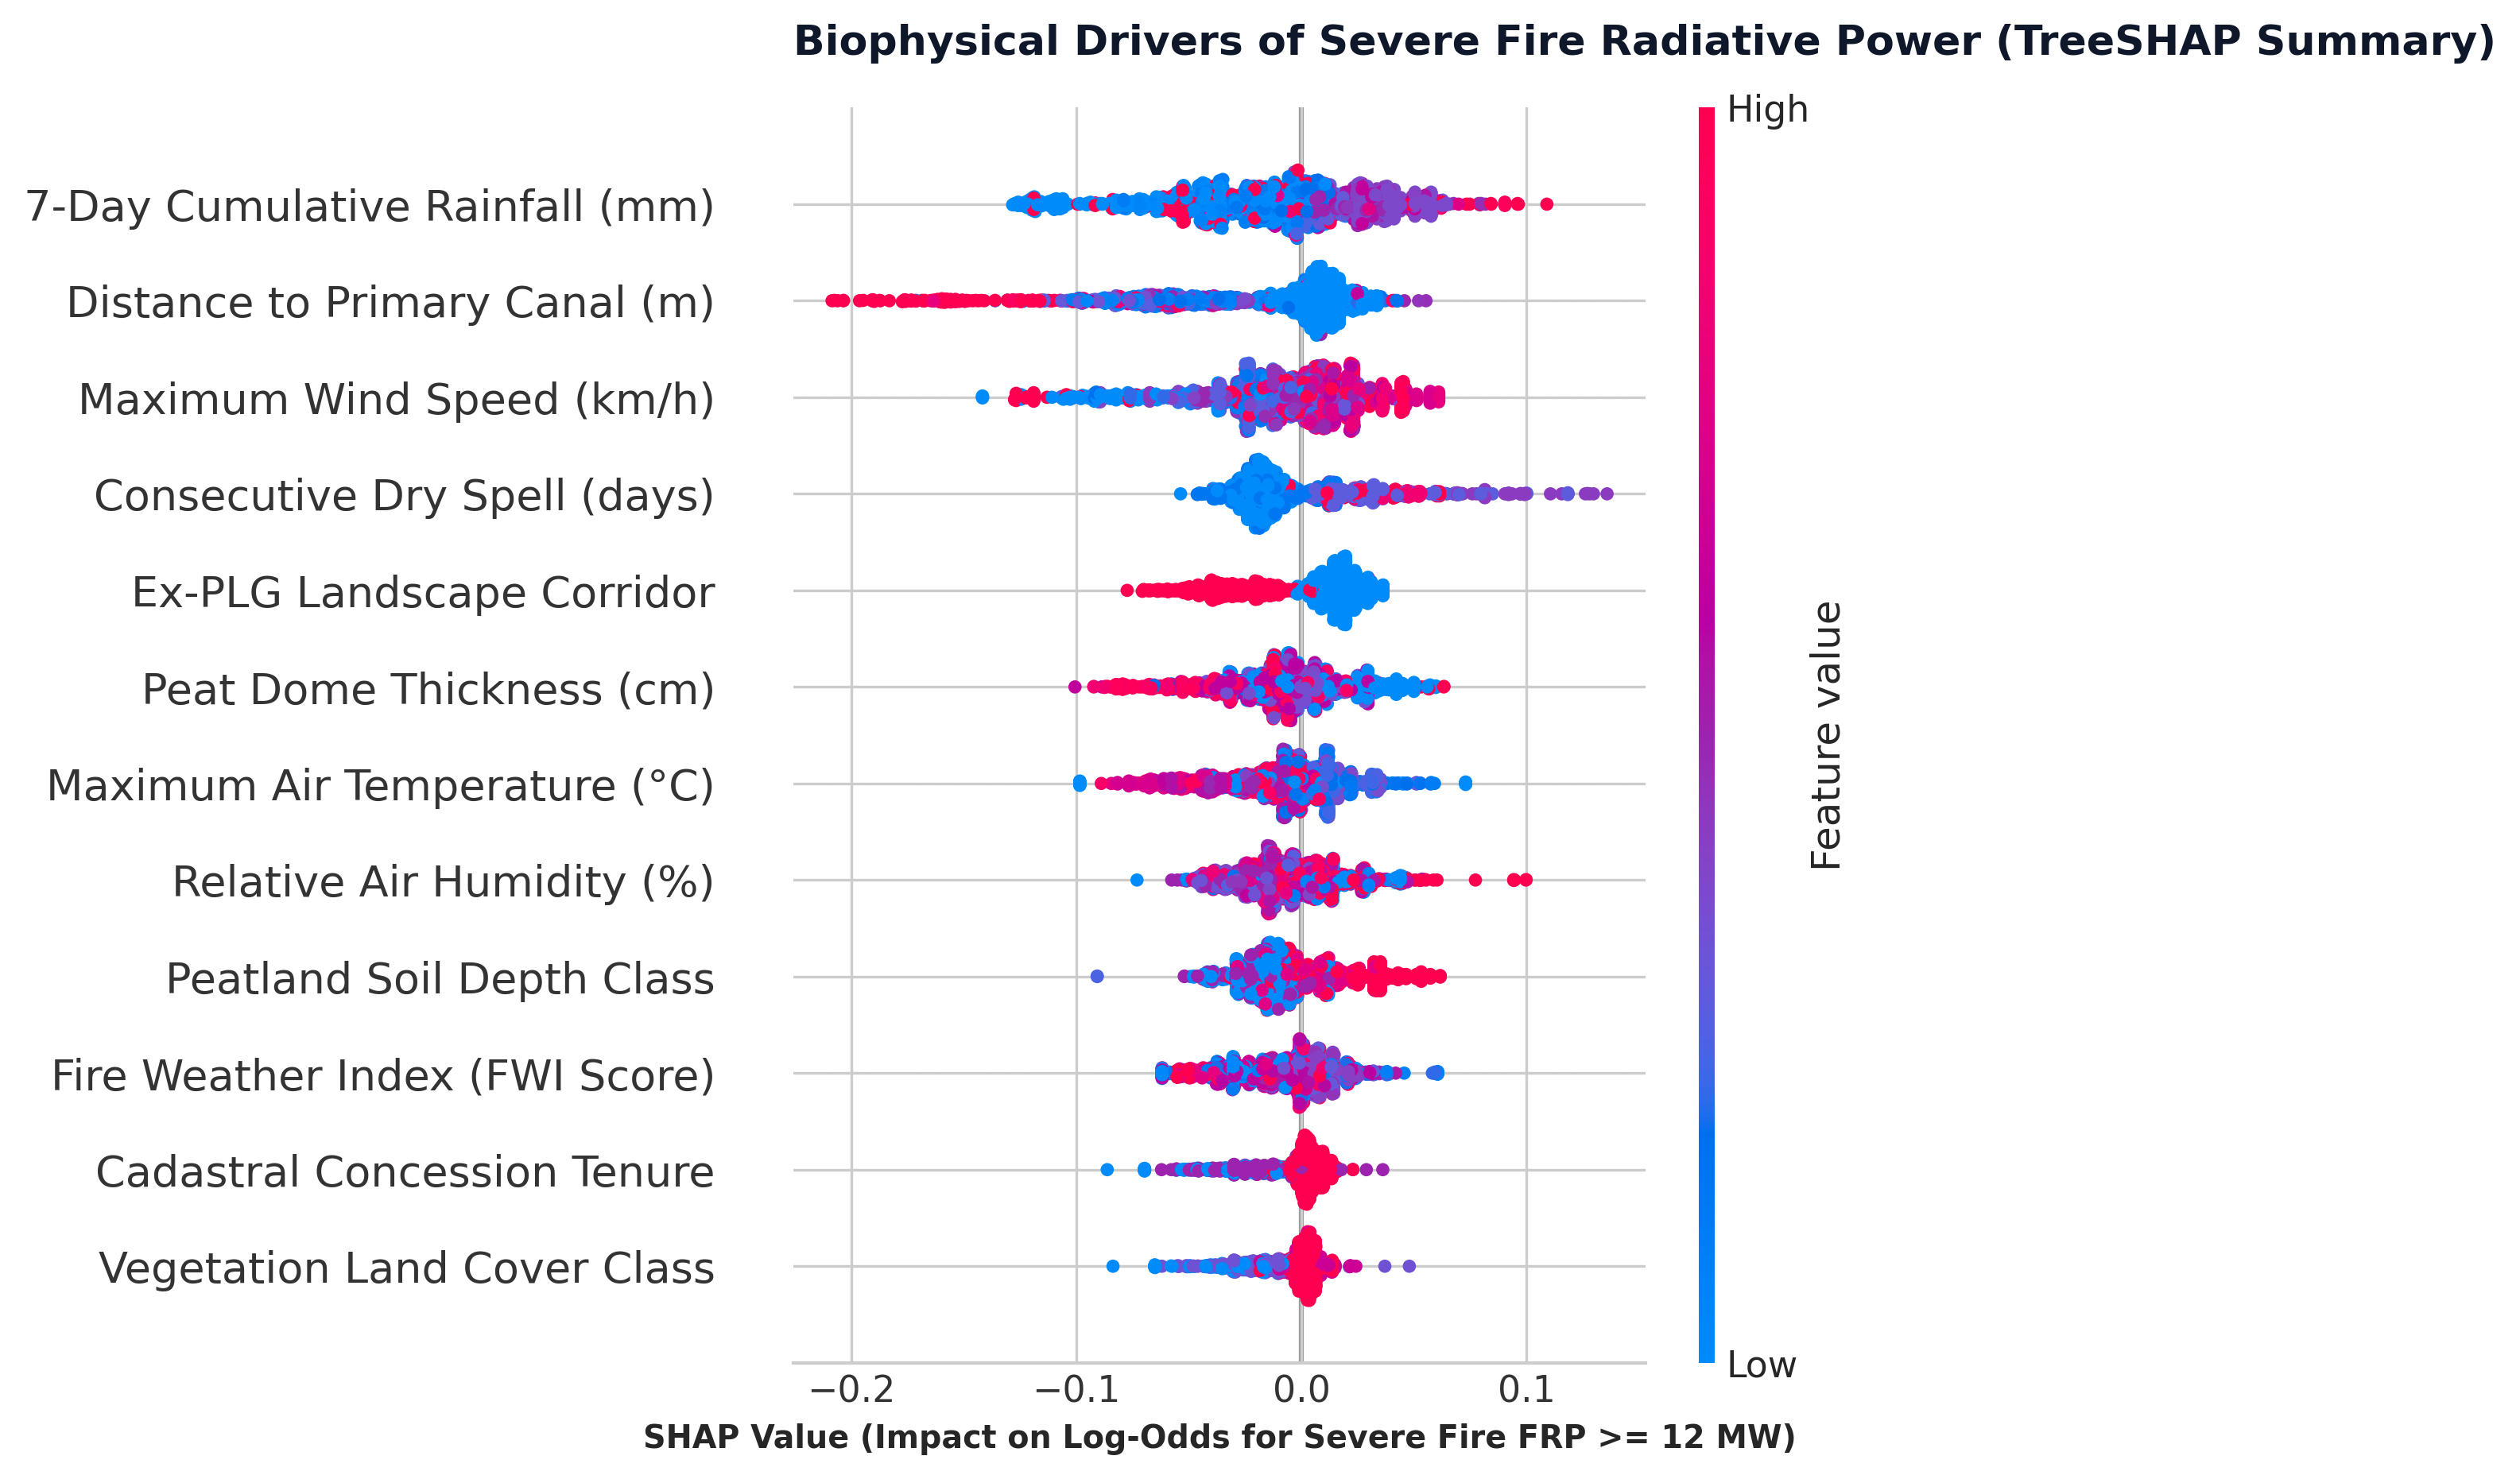
\includegraphics[width=0.92\textwidth]{07_shap_feature_importance.png}
\caption{\textbf{TreeSHAP summary beeswarm plot for Model B.} Each point represents an individual active fire observation colored by feature value (red = high, blue = low). The distribution uncovers critical non-linear thresholds: 7-day antecedent rainfall deficit ($<5$\,mm), proximity to primary drainage canals ($<3$\,km), and extended dry spells ($>14$\,days) strongly increase the log-odds of severe Fire Radiative Power ($\text{FRP} \ge 12.0$\,MW).}
\label{fig:shap_importance}
\end{figure}

The TreeSHAP beeswarm distribution showed three non-linear thresholds in fire severity:
\begin{enumerate}
    \item Rainfall Deficit: 7-day cumulative precipitation ($P_{\text{7d}}$) was the most influential predictor ($\text{mean } |\text{SHAP}| = 0.0329$). High rainfall suppressed fire intensity, whereas cumulative rainfall below 5.0\,mm increased severe fire log-odds by up to $+0.18$.
    \item Canal Proximity: In the ex-PLG landscape, proximity to primary canals ($d_{\text{canal}}$) had the second-highest attribution (0.0322). Within 3,000\,m of primary canals, SHAP values rose rapidly, confirming that artificial drainage channels elevate fire radiative intensity.
    \item 14-Day Dry Spell Threshold: Dry spell duration ($D_{\text{spell}}$) showed little positive attribution during the first 7 days of dry weather. Between 12 and 14 consecutive rainless days, SHAP values rose sharply as water tables dropped below the upper peat layer.
\end{enumerate}
